\documentclass{article}
\usepackage{graphicx}
\usepackage[utf8]{inputenc}
\usepackage{listings}
\usepackage{color}
\usepackage{xcolor}
\usepackage{textcomp}
\usepackage{amsmath}
\usepackage{mathabx}

\definecolor{solarized@base03}{HTML}{002B36}
\definecolor{solarized@base02}{HTML}{073642}
\definecolor{solarized@base01}{HTML}{586e75}
\definecolor{solarized@base00}{HTML}{657b83}
\definecolor{solarized@base0}{HTML}{839496}
\definecolor{solarized@base1}{HTML}{93a1a1}
\definecolor{solarized@base2}{HTML}{EEE8D5}
\definecolor{solarized@base3}{HTML}{FDF6E3}
\definecolor{solarized@yellow}{HTML}{B58900}
\definecolor{solarized@orange}{HTML}{CB4B16}
\definecolor{solarized@red}{HTML}{DC322F}
\definecolor{solarized@magenta}{HTML}{D33682}
\definecolor{solarized@violet}{HTML}{6C71C4}
\definecolor{solarized@blue}{HTML}{268BD2}
\definecolor{solarized@cyan}{HTML}{2AA198}
\definecolor{solarized@green}{HTML}{859900}

\lstset{
  language=Python,
  upquote=true,
  columns=fixed,
  tabsize=2,
  extendedchars=true,
  breaklines=true,
  frame=single,
  numbers=left,
  numbersep=5pt,
  rulesepcolor=\color{solarized@base03},
  numberstyle=\tiny\color{solarized@base01},
  basicstyle=\footnotesize\ttfamily,
  keywordstyle=\color{solarized@green},
  stringstyle=\color{solarized@cyan}\ttfamily,
  identifierstyle=\color{solarized@blue},
  commentstyle=\color{solarized@base01},
  emphstyle=\color{solarized@red}
}
\begin{document}

\title{Tarea 3}
\author{Angel Caceres Licona}

\maketitle


\section{Complete la tabla 1}

\begin{center}
    \begin{tabular}{||c c c c c c c||} 
    \hline
    $k$ & $a_k$ & $b_k$ & $m_k$ & $f(m_k)$ & $\frac{|m_k - a|}{|a|}$ \\ [0.5ex] 
    \hline\hline
    0 & 1.8 & 2 & 1.9 & - & 0.9025 \\ 
    \hline
    1 & 1.9 & 2 & 1.95 & + & 0.950625 \\
    \hline
    2 & 1.9 & 1.95 & 1.925 & - & 0.92640625\\
    \hline
    3 & 1.925 & 1.95 & 1.9375 & + & 0.9384765625\\
    \hline
    4 & 1.925 & 1.9375 & 1.93125 & - & 0.932431640625\\
    \hline 
    5 & 1.93125 & 1.9375 & 1.934375 & + & 0.9354516601562499\\ 
    \hline 
   \end{tabular}
\end{center}

\section{Realice un programa numérico que resuelva una exuación usando el método de bisección...}

\begin{lstlisting}
    from math import *
 

    a = float(input('Ingrese el valor a:'))
    b = float(input('Ingrese el valor b:'))
    tol = float(input('Ingrese la tolerancia:'))
    maxIter = 1000000
     
    def f(x):
        return 250*(((1+(x/12))**36-1)/(x/12)) +13500*((1+(x/12)**36))-25000
     
    i = 1
    fa = f(a)
    fb = f(b)
    print ("Iteracion     a     b     c     f(c)")
    while i <= maxIter:
        pMedio = (a + b)/2
        fc = f(pMedio)
        print( "%.7f" %i, "%.7f" %a,"    %.7f" %b,"    %.7f" %pMedio, "    %.7f" %fc)
        if (fc == 0) or abs(b - a) < tol:
            print ("La raiz buscada es: %.7f" %pMedio, "con " + str(i) + " iteraciones.")
            break
        
        i = i +1
        if (fa*fc > 0):
            a=pMedio
            fa = f(a)
    
        else:
            b = pMedio
            fb = f(b)
\end{lstlisting}
La salida del programa es la siguiente: 

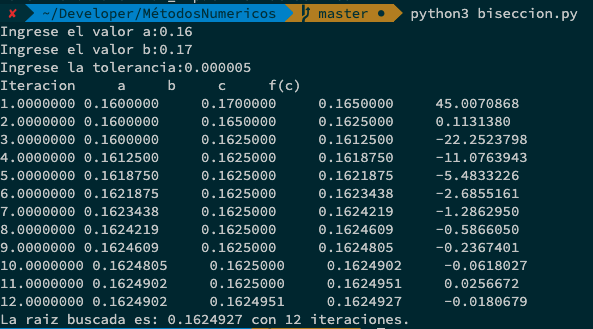
\includegraphics[scale=0.5]{salidaBiseccion.png}


\section{Grafique la funcion $f(r)$ (6) en Mathematica...}
\begin{center}
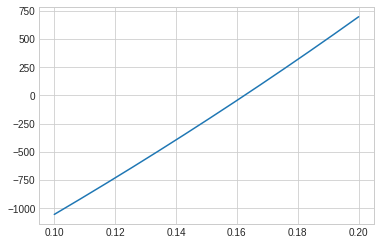
\includegraphics[scale=0.5]{plot.png}
\end{center}

Podemos ver que tiene una raiz en $\approx 0.16$

\section{Grafique la funcion $f(r)$ (6) en Mathematica...}

\begin{center}
    \begin{tabular}{||c c c c c c c||} 
    \hline
    $k$ & $a_k$ & $b_k$ & $m_k$ & $f(m_k)$ & $\frac{|m_k - a|}{|a|}$ \\ [0.8ex] 
    \hline\hline
    0 & 0.1600000 & 0.1700000 & 0.1650000 & + & 45.0070868 \\ 
    \hline
    1 & 0.1600000 & 0.1650000 & 0.1625000  & + & 0.1131380 \\
    \hline
    2 & 0.1600000 & 0.1625000 & 0.1612500 & - & -22.2523798\\
    \hline
    3 & 0.1612500 & 0.1625000 & 0.1618750 & - & -11.0763943\\
    \hline
    4 & 0.1618750 & 0.1625000 & 0.1621875 & - & -5.48332265\\
    \hline 
    5 & 0.1621875 & 0.1625000 & 0.1623438 & - & -2.6855161\\ 
    \hline 
    6 & 0.1623438 & 0.1625000 & 0.1624219 & - & -1.2862950\\ 
    \hline 
    7 & 0.1624219 & 0.1625000& 0.1624609 & - & -0.5866050\\ 
    \hline 
    8 & 0.1624609 & 0.1625000 & 0.1624805 & - & -0.2367401\\ 
    \hline 
    9 & 0.1624805 & 0.1625000 & 0.1624902  & - & -0.0618027\\ 
    \hline 
    10 & 0.1624902 & 0.1625000 & 0.1624951 & + & 0.0256672\\ 
    \hline 
    11 & 0.1624902 & 0.1624951 & 0.1624927 & - & -0.0180679\\[1ex]
    \hline
   \end{tabular}
\end{center}

\end{document}